\begin{blocksection}
\question

\textbf{\underline{Control Logic}}

A controller send signals to our circuit, telling which pieces to perform what operations.  Not all control signals matter for every instruction: for example, R-type instructions ignores the output from the immediate generator.  Control signals are used to pick between mux inputs in order to perform the correct operation.  They are embedded within the actual machine code for an instruction.

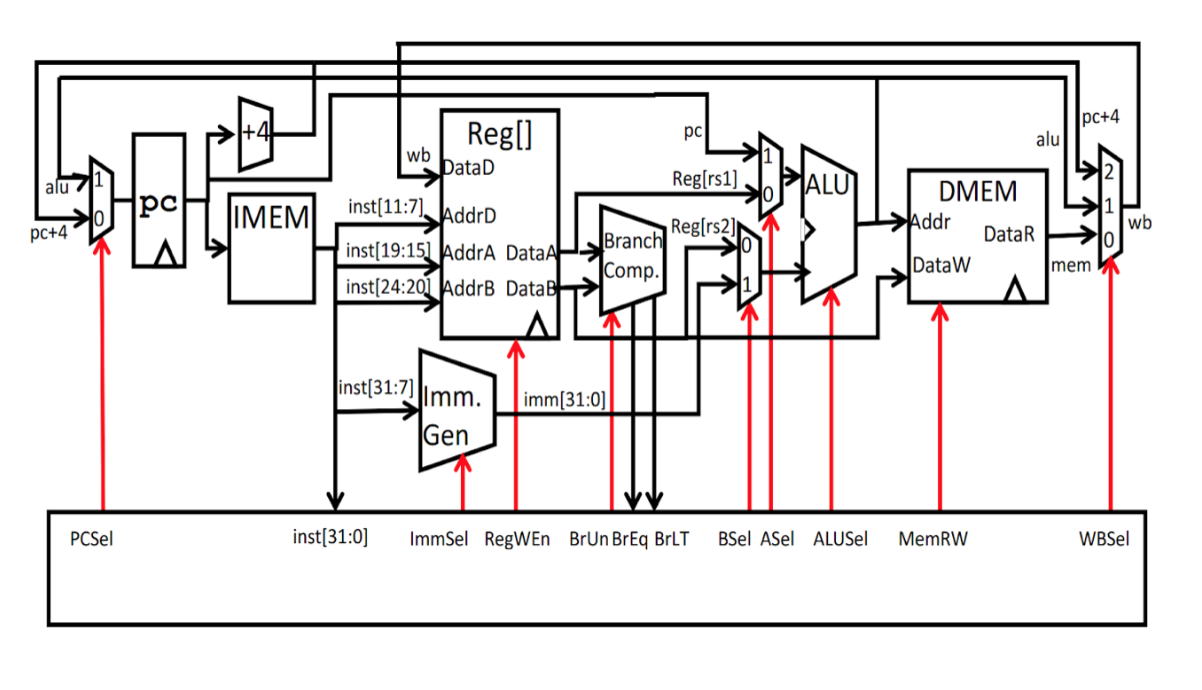
\includegraphics[width=\textwidth]{singlecycle/explanation_2}

\textbf{Control Inputs}\\\\
\begin{tabular}{ |l|l|l|l| } 
 \hline
 \textbf{Signal:} & \textbf{inst[31:0]} & \textbf{BrEq} & \textbf{BrLT} \\ 
 \hline
 Purpose: & Sends the current instruction to control & (DataA == DataB) ? 1 : 0 & (DataA < DataB) ? 1 : 0 \\ 
 \hline
\end{tabular}

\textbf{Control Outputs}\\\\
\begin{tabular}{ |l|l|l|l|l| } 
 \hline
 \textbf{Signal:} & \textbf{Purpose:} \\
 \hline
 \hline
 PCSel & Next instruction location \\
 \hline
 ALUSel & What operation to perform. \\
 \hline
 RegWEn & Do we change a register’s value? \\
 \hline
 ImmSel & Format the immediate properly.\\ 
 \hline
 MemRW & Read or write to mem. \\
 \hline
 WBSel & What value to write back. \\
 \hline 
 BrUn & Branch signed or unsigned. \\
 \hline 
 ASel/BSel & Pick between the inputs for ALU. \\
 \hline
\end{tabular}

\end{blocksection}